\documentclass[main.tex]{subfiles}

\begin{document}

\section{Experiments}

Experiments are run on the author's personal laptop, a Dell XPS3 running Ubuntu 17.04 (Zesty) with 8GB of ram, a 256GB solid state drive, and a 7th generation Intel Core i5 processor (with 4 cores at 2.5GHz).

\subsection{Overview of Experiments}
The experiments in this thesis aim to explore the performance of optimization algorithms and heuristics on realistic enough offer network models. The run-times of MAX-WEIGHT and GSC-POD pose limitaitons on the size of the experiments that can be done. See Section \ref{exp:time} below.

Three randomly generated graphs are used: RB1, BM1, and EN. They are described in the following section.

Performance is measured based on the following metrics:

\begin{itemize}
  \item (TM): Total number of ORpairs satisfactorily matched.
  \item (WT): Average wait time of ORpairs that are matched\footnote{Wait time is measured by the number of matching periods an ORpair has been through multiplied by the frequency of matching periods, step size $n_{match}$.}.
  \item (AMS): Average number of matches accepted / suggested matches.
  \item (SMS): Average size of suggested matches.
  \item (PoD): Matched task popularity measured by average product of degrees.
  \item (TH): Total number of ORpairs held.
  \item (HT): Average number of times a hanging ORpair is held.
  \item (HWT): Max wait time of a user in a held node.
\end{itemize}


TM, WT, and SMS are standard measures \cite{Dick} \cite{And1} \cite{Abb1}. AMS relates to Section \ref{sec:cyc size} on cycle size and acceptance probability: how many users were actually satisfied per user in a suggested match? The lower PoD is, the more hard-to-match ORpairs have been matched.

The first experiments explore the effect of step size, $nMatch$, and the starting size of the graph, $Ninitial$, on performance. GSC and DYN are run up to $35,000$ ORpairs to see if the graph size stabilizes. Anderson \cite{And1} find their Erdos-Renyi model reaches a steady state at around $2,000$ ORpairs and then the size does not increase much. Is there a graph size at which the performance metrics change? Which performance metrics depend on step size? These questions are important for understanding the offer network problem, as well as for choosing the scope of the following experiments.

Taking the first experiments into account, two batches of grid experiments are run on RB1: one up to $Nend = 3,400$ to test MAX-WEIGHT, MAX-2, DYN, GSC, and GSC-POD; and another up to $Nend = 15,000$ to compare DYN, GSC, GSC-POD, and MAX-2. The grid covers a range of acceptance probabilities, HOR or not, and a smaller range of step sizes, $nMatch$.

Due to limited time, only 6 batches sampled from the grid experiments are run on EN and BM1 to check whether the results are graph specific.

Last the relation between acceptance probability and TM is examined.

Note there are more plots than needed to analyse the results. These are included in the Supplementary Materials Appendix \ref{appendix}.

\subsection{Graph Parameters}
This section describes some graph parameters used in the below experiments.

Three randomly generated graphs are used. Graph (RB1) has task degree distribution similar to Ratebeer. The average difference in in and out degrees of tasks is $1.45$, meaning that while the distributions are different, in general popular tasks are popular to both offer and request. See the graph in Figure \ref{fig:RB1}\footnote{The graphs plotted in this section have been grown to 10,000 ORpairs.} Graph (BM1) has a difference in power-law exponents similar to that of Bookmooch. The average difference is $1.42$. Graph (EN) with almost equal power-law exponents for offers and requests. The average difference is $1.36$.


\begin{center}
  \underline{RB1 parameters}

  \begin{tabular}{| c | c | c | c | c | c | }
    \hline
    $\alpha$ & $\gamma$ & $\beta$ & $p_d$ & $\delta_{in}$ & $\delta_{out}$ \\ \hline
    $0.35$ & $0.15$ & $0.5$ & $0.05$ & $1.0$ & $0.5$ \\
    \hline
  \end{tabular}
\end{center}

\begin{center}
  \underline{BM1 parameters}

  \begin{tabular}{| c | c | c | c | c | c | }
    \hline
    $\alpha$ & $\gamma$ & $\beta$ & $p_d$ & $\delta_{in}$ & $\delta_{out}$ \\ \hline
    $0.52$ & $0.12$ & $0.35$ & $0.05$ & $0.25$ & $0.05$ \\
    \hline
  \end{tabular}
\end{center}

\begin{center}
  \underline{EN parameters}

  \begin{tabular}{| c | c | c | c | c | c | }
    \hline
    $\alpha$ & $\gamma$ & $\beta$ & $p_d$ & $\delta_{in}$ & $\delta_{out}$ \\ \hline
    $0.52$ & $0.12$ & $0.35$ & $0.05$ & $0.25$ & $0.05$ \\
    \hline
  \end{tabular}
\end{center}

\begin{figure}[H]
  \centering
  \begin{minipage}[b]{0.45\textwidth}
    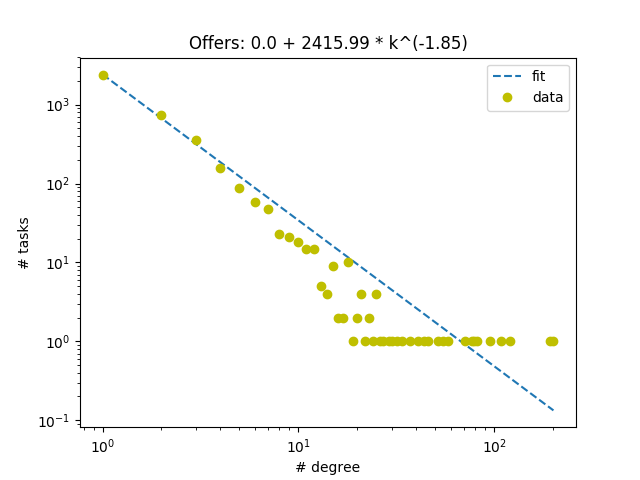
\includegraphics[width=\textwidth]{graphOffersRB.png}
    \caption{RB1 task offer distribution}
  \end{minipage}
  \hfill
  \begin{minipage}[b]{0.45\textwidth}
    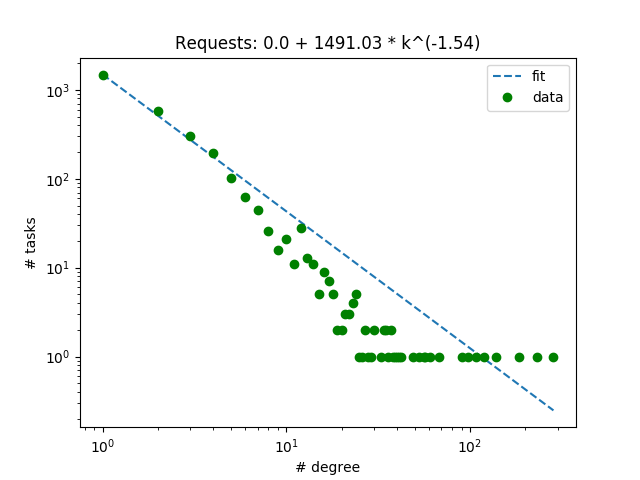
\includegraphics[width=\textwidth]{graphRequestsRB.png}
    \caption{RB1 task request distribution}
  \end{minipage}
  \label{fig:RB1}
\end{figure}

\begin{figure}[H]
  \centering
  \begin{minipage}[b]{0.45\textwidth}
    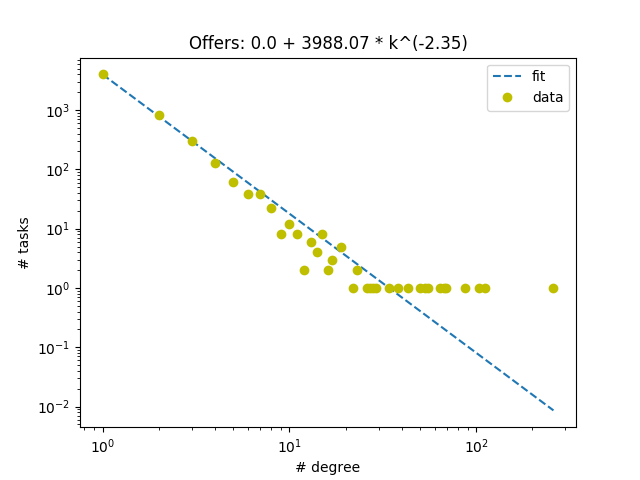
\includegraphics[width=\textwidth]{graphOffersBM.png}
    \caption{BM1 task offer distribution}
  \end{minipage}
  \hfill
  \begin{minipage}[b]{0.45\textwidth}
    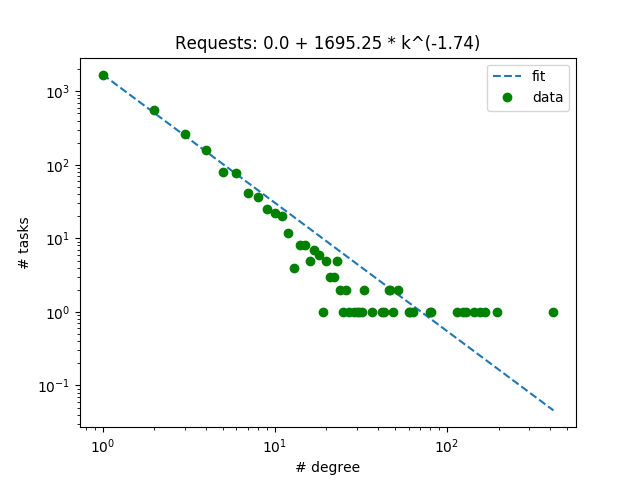
\includegraphics[width=\textwidth]{graphRequestsBM.png}
    \caption{BM1 task request distribution}
  \end{minipage}
\end{figure}

\begin{figure}[H]
  \centering
  \begin{minipage}[b]{0.45\textwidth}
    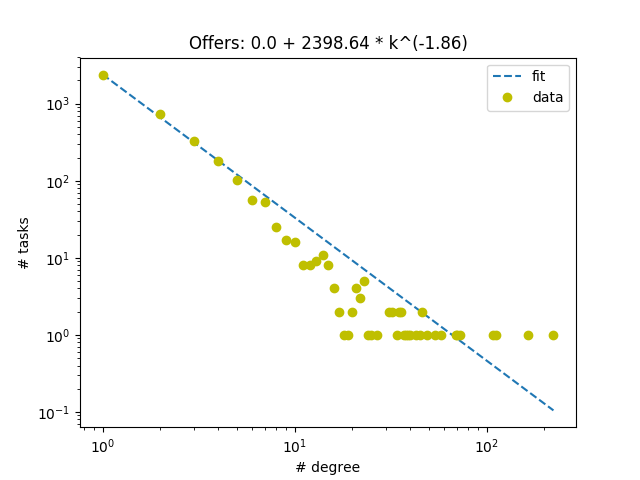
\includegraphics[width=\textwidth]{graphOffersEN.png}
    \caption{EN task offer distribution}
  \end{minipage}
  \hfill
  \begin{minipage}[b]{0.45\textwidth}
    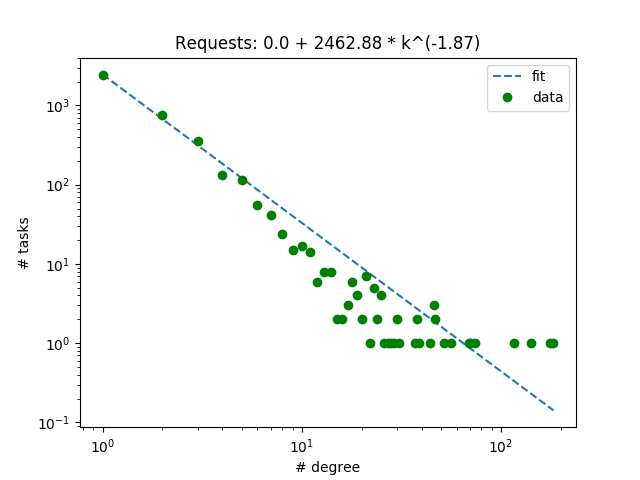
\includegraphics[width=\textwidth]{graphRequestsEN.png}
    \caption{EN task request distribution}
  \end{minipage}
\end{figure}

\subsection{Graph Generation}
For each experiment a series of graph updates is computed using the model in section \ref{sec:model}. This series is is used for each test in a single experimental run to isolate variance in the run. However, a new series is generated with the same parameters in different experiments to minimize dependence of results on any one randomly generated graph.

The matching algorithm is run after $N_{initial}$ ORpairs are added and their statistics are not preserved. Wait time counts are set to $-1$. This trade-off allows the performance at any given point in the offer network's evolution to be better tested. See Section \ref{exp:ninitial}.

\subsection{Run Time} \label{exp:time}
Each of the 4 tests below are run on different graph update series.

DYN, TWO, and GSC are run on RB1, BM1, and EN with $N_{initial} = 100$, $N_{end} = 15,000$, $n_{match} = 100$, and $p=1$ to measure match time as a function of the number of ORpairs in the graph. See Figure \ref{fig:time1}. GSC and GSC-POD are then run with the same settings in Figure \ref{fig:time3}. DYN and CSC are also run with $n_{match} = \{1, 20\}$ in Figure \ref{fig:time2}. The time test including MAX-WEIGHT, being slower, is only run up to $N_{end} = 5000$: Figure \ref{fig:time4}.

DYN, TWO, GSC, and GSC-POD all run in linear time with respect to the graph size, and MAX-WEIGHT runs in $\bO(N^3)$ time. In practice, the time to find shortest cycles seems to depend on step size \footnote{Note this could be tested more rigorously.}.

GSC is comparable to TWO. DYN scales very well with graph size compared to GSC, as performance largely depends on the number of newly adde nodes. GSC-POD scales worse, reaching $60$ seconds while $GSC$ runs in $1.5$.

\begin{figure}[H]
  \centering
    \includegraphics[width=\textwidth]{{"timeTest-EN 100"}.png}
    \caption{EN - Run Time - Step Size 100}
    \label{fig:time1}
\end{figure}
\begin{figure}[H]
    \includegraphics[width=\textwidth]{{"timeTest-RB1 100-2"}.png}
    \caption{RB1 - Run Time - GSC-POD}
    \label{fig:time3}
\end{figure}
\begin{figure}[H]
    \includegraphics[width=\textwidth]{{"timeTest-RB1 20"}.png}
    \caption{RB1 - Run Time - Step Size 20}
    \label{fig:time2}
\end{figure}
\begin{figure}[H]
    \includegraphics[width=\textwidth]{{"timeTest-RB1 100-MAX"}.png}
    \caption{RB1 - Run Time - MAX-WEIGHT}
    \label{fig:time4}
\end{figure}

\subsection{Effect of step size, $n_{match}$, on performance} \label{exp:nmatch}
The matching algorithms (GSC, DYN, MAX-WEIGHT, MAX-2) are run on $n_{match} \in \{5, 10, 20, 40, 80, 120, 240, 480, 960\}$ with $N_{initial} = 100$, $N_{end} = 3003$, and $p = 1$. Initially, I generated a graph series for each matching algorithm run, which can be seen in Figures \ref{fig:nMatch1} and \ref{fig:nMatch2}.

Note that in the first run TM (toal matched) does not depend much on match frequency MAX-WEIGHT, which can have very high match sizes has a small average MS comparable to the short cycle seeking algorithms. MAX-2 performs the same regardless of the match size, implying there are limtied 2-way swaps.

GSC and DYN performance decreases slightly with match frequency. MAX-WEIGHT's performance increases, but this comes at the cost of more than doubling the WT (wait time).

Another run where all matching algorithms are tested on the same generated graph series is done with $p=1$, $N_{initial} = 100$, $N_{end} = 5000$, and $n_{match} \in \{1, 2, 3, 4, 5, 10, 20, 40, 60, 80, 100, 125, 250, 500, 1000\}$. See Figures \ref{fig:nMatch3} and \ref{fig:nMatch4}. The variance in performance diminishes.

The experiments show that the particular step size does not matter much for performance, provided $n_{match} \leq 50$, moreover MAX-WEIGHT may perform comparably to GSC and DYN with low acceptance probability $p$

Unfortunately\footnote{As the author does not have time to add a more nuanced wait time measurement.}, the way WT is measured, an ORpair added $i$ steps before matching will be assumed to have waited for roughly $n_{match} - i$ steps longer than it has. This will lead to an average error of roughly a $n_{match}/2$ longer average wait time. The effect will be more pronounced when $(N_{end} - N_{initial}) / n_{match}$ is small. This correction seems to bring the WT for high step sizes to par, or only a couple hundred steps, higher than for low step sizes. This implies that, contrary to expectations and the Erdos-Renyi model in Anderson \cite{And1}, small step sizes ($n_{match} \leq 50$) do not out-perform large ones much.

Interestingly, $n_{match} = {10, 20}$ can outperform $n_{match} = {5}$ on both WT and TM metrics.

\begin{figure}[H]
    \includegraphics[width=\textwidth]{{"nMatch-BM1 "}.png}
    \caption{BM1 - Step Size Test 1 \\ The dashed lines are the WT of unmatched ORpairs, and the solid lines matched ORpairs.}
    \label{fig:nMatch1}
\end{figure}
\begin{figure}[H]
    \includegraphics[width=\textwidth]{{"nMatch-RB1 "}.png}
    \caption{RB1 - Step Size Test 1}
    \label{fig:nMatch2}
\end{figure}

\begin{figure}[H]
    \includegraphics[width=\textwidth]{{"nMatch 2-RB1 "}.png}
    \caption{RB1 - Step Size Test 2}
    \label{fig:nMatch3}
\end{figure}
\begin{figure}[H]
    \includegraphics[width=\textwidth]{{"nMatch 2-EN "}.png}
    \caption{EN - Step Size Test 2}
    \label{fig:nMatch4}
\end{figure}

\subsection{Graph Size Over Time} \label{exp:gsize}
DYN is run on RB1, BM1, and EN from $100$ to $35,000$ ORpairs with $p=1$ and $nMatch = 20$. GSC is also run on EN.
The graph size grows linearly in added ORpairs, with a coefficient less than one.

\begin{figure}[H]
    \includegraphics[width=\textwidth]{{"timeSeries"}.png}
    \caption{Graph Size vs ORpairs Added}
    \label{fig:gsize}
\end{figure}

\subsection{Effect of initial graph size, $N_{initial}$, on performance} \label{exp:ninitial}
Matching algorithms (TWO, DYN, GSC) are run for $3000$ steps starting at $N_{initial} \in$ \{10, 50, 100, 200, 400, 600, 800, 1000, 1200, 1600, 2000, 3000, 4000, 5000, 6000, 7000, 8000, 9000, 10000, 11000\} with step size $n_{match} = 20$ and $p=1$. \footnote{The graph sizes are too big for MAX-WEIGHT, but the trends likely to be similar. It's possible, however, MAX-WEIGHT will take better advantage of larger graph size.}

The TM (total matched) ORpairs is near constant for DYN and GSC, and decresase for TWO. MS (match size) increases, more for GSC, with graph size. Matched and unmatched WT (wait time) rapidly increases and appears to level off to around double the low $N_{initial}$ WT. Thus a stable state with respect to throughput\footnote{Through put is the number of matched ORpairs in a given timeframe, that is, TM and WT} seems to be reached for $N_{initial} > 10,000$. As in Section \ref{exp:gsize} the graph size does not stabilize, this is likely a balance of two factors:

\begin{itemize}
  \item There are more ORpairs to be matched with as graph size increases.
  \item There are fewer cycles containing any two non-popular nodes as graph size increases.
\end{itemize}

First, it's worth doing experiments with large enough graphs that wait time has leveled off.

However, this is not feasible with MAX-WEIGHT. Fortunately, the dependence on $N_{initial}$ appears uniform among matching algorithms.

\begin{figure}[H]
    \includegraphics[width=\textwidth]{{"Ninitial-EN "}.png}
    \caption{Ninitial Test - EN}
    \label{fig:ninitial}
\end{figure}

\subsection{Performance Test -- Low $N_{initial}$} \label{exp:ptest1}
This experiment is run from $N_{initial} = 400$ to $N_{end} = 3400$. Without the HOR approach with held ORpairs only $p=0.9$ is tested. With HOR, $p \in \{0.3, 0.5, 0.7, 0.8, 0.9\}$ are tested.

The matching algorithms are run with the following step size values:

\begin{center}
  %\underline{BM1 parameters}
  \begin{tabular}{| c | l | }
    \hline
    Matching Algorithm & $n_{match}$ \\ \hline
    GSC & \{1, 5, 10, 25, 50, 100, 250\} \\ \hline
    DYN & \{1, 5, 10, 25, 50, 100, 250\} \\ \hline
    GSC-POD & \{5, 10, 25, 50, 100, 250\} \\ \hline
    MAX-2 & \{5, 10, 25, 50, 100, 250\} \\ \hline
    MAX-WEIGHT & \{40, 100, 250, 500\} \\
    \hline
  \end{tabular}
\end{center}

For the plots in this and the following section, remember that solid lines for wait time, task popularity (measured by PoD, product of degrees), and hold times. Total matched (solid) and total held (dashed) ORpairs are shown on the same plot. SMS (average suggested match size -- solid) and AMS (average accepted matche size / SMS -- dashed) in the Match Size plot.

First, see Figure \ref{fig:ptest1} for the case without HOR. MAX-WEIGHT performs significantly worse than the other algorithms o all metrics. As indicated in MS, AMS is low. Recall that the expected number of satisfied users is: $\E[c_k] = k (0.9)^k$, and in Section \ref{exp:nmatch} MAX-WEIGHT's MS increases rapidly with match frequency. Thus even though SMS is not much higher than for GSC at low $n_{match}$, each rejected cycle will engender the same effect as having a larger $n_{match}$, a vicious cycle \footnote{It's possible for $n_{match} \leq 10$, MAX-WEIGHT will perform well. The algorithm is, however, too slow for matching every new ORpair to be considered seriously.}. No further experimentation is needed for MAX-WEIGHT without HOR. The other algorithms will be tested without HOR on larger graphs.

\begin{figure}[H]
    \includegraphics[width=\textwidth]{{"Ptest-RB1 p=0.9, hold=0"}.png}
    \caption{Performance Test - RB1 - $p = 0.9$ without HOR}
    \label{fig:ptest1}
\end{figure}

The trend in MAX-WEIGHT's performance as $p$ decreases can be seen in Figures \ref{fig:ptest2} - \ref{fig:ptest6}

\begin{figure}[H]
    \includegraphics[width=\textwidth]{{"Ptest-RB1 p=0.9, hold=1"}.png}
    \caption{Performance Test - RB1 - $p = 0.9$ with HOR}
    \label{fig:ptest2}
\end{figure}

At $p = 0.9$, MAX-WEIGHT and HOR outperforms the other algorithms in TM, WT, and PoD. HWT (hold wait time) is only about $1.5$ times the average wait time, and nodes are held more than once are rare. Larger match sizes seem okay.

\begin{figure}[H]
    \includegraphics[width=\textwidth]{{"Ptest-RB1 p=0.8, hold=1"}.png}
    \caption{Performance Test - RB1 - $p = 0.8$ with HOR}
    \label{fig:ptest3}
\end{figure}

\begin{figure}[H]
    \includegraphics[width=\textwidth]{{"Ptest-RB1 p=0.7, hold=1"}.png}
    \caption{Performance Test - RB1 - $p = 0.7$ with HOR}
    \label{fig:ptest4}
\end{figure}

At $p = 0.8$ and $p = 0.7$, MAX-WEIGHT performs on par with generally better PoD. AMS decreases, and more nodes are held. HWT about $2$ times WT.

\begin{figure}[H]
    \includegraphics[width=\textwidth]{{"Ptest-BM1 p=0.5, hold=1"}.png}
    \caption{Performance Test - BM1 - $p = 0.5$ with HOR}
    \label{fig:ptest5}
\end{figure}

\begin{figure}[H]
    \includegraphics[width=\textwidth]{{"Ptest-EN p=0.3, hold=1"}.png}
    \caption{Performance Test - EN - $p = 0.3$ with HOR}
    \label{fig:ptest6}
\end{figure}

At $p = 0.5$ and $p = 0.3$, GSC out-performs MAX-WEIGHT: short cycles become important in spite of HOR. By $p = 0.3$, held nodes are held for an average of $4.5$ rounds. Interestingly, despite performing worse, MAX-WEIGHT achieves better PoD. This may be due to the \textit{optimality} of the suggestsed matching. Note also that AMS gets very low, near zero, even for GSC.

Another trend is that small step sizes performs increasingly well as $p$ decreases: with high cycle rejections and held ORpairs, there are more often potential matches. Thus suggesting matches with high frequency works well.

This experiment batch shows that HOR can be an effective approach and workaround to mid and high $p \geq .07$. MAX-WEIGHT, which performs dismally without HOR, performs better than the other matching algorithms with HOR. Even in low $p$ ranges, MAX-WEIGHT only matches a couple hundred fewer ORpairs than GSC and has comparable wait time.


\subsection{Performance Test -- High $N_{initial}$} \label{exp:ptest2}
This experiment, without MAX-WEIGHT, is run from $N_{initial} = 10,000$ to $N_{end} = 15,000$. The bulk of the experiment is done on RB1, with 2 on EN and 2 on BM1 to verify that the results do not depend on the specifics of RB1. Without holding ORpairs, $p \in \{0.3, 0.5, 0.7, 0.9\}$; and with HOR, $p \in \{0.3, 0.5, 0.6, 0.7, 0.8, 0.9\}$.

The matching algorithms are run with the following step size values:

\begin{center}
  %\underline{BM1 parameters}
  \begin{tabular}{| c | l | }
    \hline
    Matching Algorithm & $n_{match}$ \\ \hline
    GSC & \{1, 5, 25, 50, 100\} \\ \hline
    DYN & \{1, 5, 25, 50, 100\} \\ \hline
    GSC-POD & \{50, 100\} \\ \hline
    MAX-2 & \{5, 25, 100\} \\
    \hline
  \end{tabular}
\end{center}

MAX-2 is only run for $p < 0.7$; however its performance is always dismal.

\subsubsection{Acceptance Probability and Performance}
The following plot is made with the best performing matching algorithm's best $n_{match}$ setting where $0$ is without HOR and $1$ is with HOR.

\begin{figure}[H]
    \includegraphics[width=\textwidth]{{"PvTM"}.png}
    %\caption{p vs TM}
    \label{fig:pvtm}
\end{figure}

First, note that even without HOR, the best performance is achieved with $p=0.7$ and $p=0.5$! This result is surprising. Randomly rejecting matches with high probaility ($98\%$ chance of rejection for 10-cycles at $p=0.7$) may be harnessing some of the effect Dickerson \cite{Dick} noted with vertex/edge/cycle/graph potentials. However, the way these are utilized seems to be by repeatedly trying larger matches until one gets lucky, which is only a feasible strategy is querying users' acceptance is cheap.

With HOR, TM and WT improve as $p$ decreases, as does GSC-POD's relative performance and PoD. The relative advantage of low step sizes diminishes. A popular task can, via being held or rejected, facilitate multiple exchanges before being part of an accepted ORpair. Curiously, these results imply that for high $p$ randomly rejecting some suggested matches could be a good heuristic, very reminiscent of Dickerson's potentials method.

While HOR's best performance is higher than without, curiously, HOR seems counterproductive at high $p$ values. With HOR when a user rejects a match, 3 users go unsatisfied in that round. It seems that with $p=0.9$ simply rejecting and finding a new match is better. As seen later in Figure \ref{ptest01}, the average match size for GSC-POD at $n_{match} = 50$ is 10, the optimal for $p=0.9$ with an expected number of satisfied users of $3$\footnote{Dicussed in Section \ref{sec:cyc size}}.

\subsubsection{Without HOR}

First note that trend of small $n_{match}$ performing better as $p$ decreases holds for high $N_{initial}$ too without HOR in Figures \ref{fig:ptest01} - \ref{fig:ptest04}

\begin{figure}[H]
    \includegraphics[width=\textwidth]{{"Ptest2-RB1 p=0.9, hold=0"}.png}
    \caption{Performance Test - RB1 - $p = 0.9$ without HOR}
    \label{fig:ptest01}
\end{figure}

As in the $p=1$ case, step size does not matter much and GSC, DYN, and GSC-POD perform about equally. GSC matches more unpopular tasks despite GSC-POD prioritizing them: perhaps in the scale free graph unpopular tasks are more likely to be connected to popular tasks?

\begin{figure}[H]
    \includegraphics[width=\textwidth]{{"Ptest2-RB1 p=0.7, hold=0"}.png}
    \caption{Performance Test - RB1 - $p = 0.7$ without HOR}
    \label{fig:ptest02}
\end{figure}

Step-size starts becoming significant. Oddly, GSC ends up with very high SMS (suggested match sizes): GSC-POD performs better even with $n_{match} = 50$. Both have as good WT as with $p=0.9$, despite the AMS being near zero instead of 3 (that is, on average a suggested match resulted in 3 satisfied ORpairs). First, this means many more matches are being suggested. The thicker graph then semes to allow ORpairs to get matched as fast despite multiple attempts being needed on average.

DYN starts performing poorly. This is likely because rejected ORpairs are not treated as new nodes by the dynamic matching.

\begin{figure}[H]
    \includegraphics[width=\textwidth]{{"Ptest2-RB1 p=0.5, hold=0"}.png}
    \caption{Performance Test - RB1 - $p = 0.5$ without HOR}
    \label{fig:ptest03}
\end{figure}

Indications are GSC-POD would out-perform GSC if run with smaller step size; however, even at large step size, GSC has better WT.

\begin{figure}[H]
    \includegraphics[width=\textwidth]{{"Ptest2-RB1 p=0.3, hold=0"}.png}
    \caption{Performance Test - RB1 - $p = 0.3$ without HOR}
    \label{fig:ptest04}
\end{figure}

GSC performs significantly better than GSC-POD. The WT, however, has doubled or tripled: very many matches are needed to get an accepting match, which doesn't happen unless step size is small.


\subsubsection{With HOR}

\begin{figure}[H]
    \includegraphics[width=\textwidth]{{"Ptest2-RB1 p=0.9, hold=1"}.png}
    \caption{Performance Test - RB1 - $p = 0.9$ with HOR}
    \label{fig:ptest11}
\end{figure}

As in the $p=1$ case, step size does not matter much and GSC, GSC-POD perform about equally.

DYN already performs worse: likely because held nodes are not treated as newly added nodes.

\begin{figure}[H]
    \includegraphics[width=\textwidth]{{"Ptest2-RB1 p=0.8, hold=1"}.png}
    \caption{Performance Test - RB1 - $p = 0.8$ with HOR}
    \label{fig:ptest12}
\end{figure}

Same as with $p=0.8$, except GSC-POD has slightly better PoD.

\begin{figure}[H]
    \includegraphics[width=\textwidth]{{"Ptest2-RB1 p=0.7, hold=1"}.png}
    \caption{Performance Test - RB1 - $p = 0.7$ with HOR}
    \label{fig:ptest13}
\end{figure}

GSC-POD's PoD advantage increases slightly.

\begin{figure}[H]
    \includegraphics[width=\textwidth]{{"Ptest2-RB1 p=0.6, hold=1"}.png}
    \caption{Performance Test - RB1 - $p = 0.6$ with HOR}
    \label{fig:ptest14}
\end{figure}

GSC-POD's PoD performance increases even more.

\begin{figure}[H]
    \includegraphics[width=\textwidth]{{"Ptest2-RB1 p=0.5, hold=1"}.png}
    \caption{Performance Test - RB1 - $p = 0.5$ with HOR}
    \label{fig:ptest15}
\end{figure}

GSC-POD's TM may be slightly better than GSC's now.

\begin{figure}[H]
    \includegraphics[width=\textwidth]{{"Ptest2-RB1 p=0.3, hold=1"}.png}
    \caption{Performance Test - RB1 - $p = 0.3$ with HOR}
    \label{fig:ptest16}
\end{figure}

GSC-POD's TM trajectory slightly higher than GSC's, and PoD performance significantly better. GSC-POD seems to perform best with low $p$ and HOR, perhaps because this leads to hard-to-match tasks being shuffled around more.

Small step size does not confer much performance benefit for $p \geq 0.5$. This is promising as algorithms such as GSC-POD that take additional factors into account are slower (even if still linear in the graph size). This can also be because new nodes are created with HOR, and thus the same cycle can't be repeated over and over again \footnote{However, a held ORpair could be matched up in a 2-cycle with the rejecting ORpair that triggered its formation. Both fortunately and interestingly, this does not seem to be happening excessively. An algorithm that abused this lazy implementation feature could suggest the same matches as for $p=1$, and then \textit{fill in the gaps} in the next few rounds by suggesting this 2-cycle until it's accepted. Yet this alone would lead to the same performance as with $p=1$, except longer delays in hold wait time (HWT). The average HWT is around 1.5x to 2x the average wait time (WT), indicating held ORpairs are actually rematched. Moreover, total matched (TM) and WT performance are actually \textit{better} with mid-$p$ ranges. So it would appear there is more going on.}

Wait time trends are interesting: WT decreases with $p$ from $0.9$ to $0.5$ and HWT increases as $p$ decreases. HWT does not increase much over the WT of about 1000 for $p \geq 0.9$. This supports the increased dynamism hypothesis behind higher performance for lower $p$.

\end{document}
